%\begin{figure}[h]
%\hspace*{\fill}
%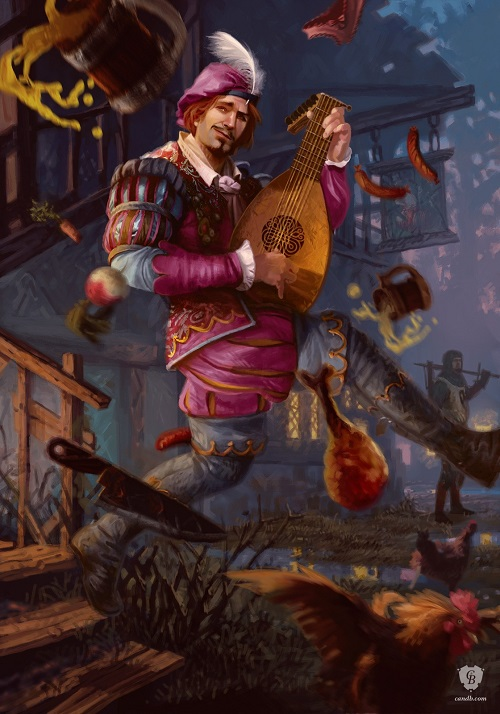
\includegraphics[width=\linewidth,natwidth=350,natheight=499]{L.jpg}
%\hspace*{\fill}
%\end{figure}

Лютик в своей жизни слишком часто занимал деньги у друзей, знакомых и не самых прияных личностей. 
Чаще всего он одолживал кругленькую сумму у очень влиятельного человека, не будем раскрывать его личность, чтобы не порочить его доброе имя. 
Но все хорошее когда-то заканчивается и в один солнечный день пришло время платить. Лютик как обычно сидел в таверне, тихо напевал под нос веселенькую песенку и радовался жизни, 
как вдруг дверь кабака с грохотом отворилась и в помещение зашло два огромных амбала, которые прямиком направились к нашему герою. Они схватили его и потащили к своему господину. 
Что произошло дальше история умалчивает, а мы вернемся к нанему барду через несколько дней.   
\\
...
\\ 
Через несколько дней Лютик с больим фингалом под правым глазом и разбитой губой сидел в доме Золтана и просил у него помощи. Ему необзодимо было вернуть все деньги, что он занимал.
К сожалению память никогда не была сильной стороной барда и он не помнил точную сумму долга. 
Но он точно помнил, что в четные дни он занимал деньги по одному правилу, а в нечетные  - по-другому. 
Хорошо подумав, он вспомнил эти правила. Они получились следующими:
\begin{equation*}
A[0]=A[1]=1
\end{equation*}
\begin{equation*}
A[2n]=A[n]+A[n-1]
\end{equation*}
\begin{equation*}
A[2n+1]=A[n]-A[n-1]
\end{equation*}
Помогите Лютику узнать, сколько денег ему нужно вернуть, если он точно знает, что n дней назад он брал займ в первый раз. 

\InputFile
На вход подается натуральное число $n$ ($0 < n < 40$)~---~количество дней, за которое копится долг.

\OutputFile
Помогите Лютику найти сумму долга, а именно $n$-й член данной последовательности.

\SAMPLES